%
\chapter{Fundamentals}\label{cha:Fundamentals}
%
In this chapter, the fundamentals of lane detection will be explained. All methods, which are used in this thesis, will be theoretically focused and the use of their functions in software will be also explained. Also, some advantages and disadvantages of methods will be discussed.
%
\section{Properties of Truck at Carola-Cup}\label{sec:Properties of Truck at Carolo-Cup}
%
The Carolo-Cup is an annual competition at the Technical University of Braunschweig which are attended by students. Every year the truck and some properties of the competition are changing. For example, in the competitions until 2017 there was no traffic sign, but starting in 2017 there are also some traffic signs, speed limit zones, blocked areas and crosswalks for pedestrian. Because of this, in the competitions until 2017, there was only one way to understand who had the right of way. If there is a stop line on the road in front of an intersection, it means the car has to wait until the intersection is free. In the competitions starting from 2017, the intersections are in different parts: They are 'Intersections with stop lines', 'Intersections with give-way lines', 'Intersections with priority to right', 'Enforced crossing direction - give-way condition', 'Enforced crossing direction - right of way condition'. Except 'Intersections with priority to right', they all have traffic signs stating who has priority. If there is a no traffic sign, it means the right side always has priority.\cite{Carolo_Cup}

\begin{figure}[H]
	\centering
	\hspace*{0cm}   
	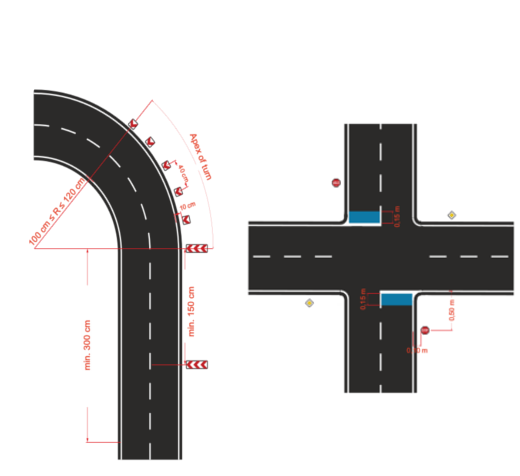
\includegraphics[width=120mm,scale=1]{./Bilder/Intersections.png}
	\caption{Left: Markings for sharp turns at Carolo-Cup.
Right: Intersections with stop lines at Carolo-Cup\cite{Carolo_Cup}}
\end{figure}



%
\section{Inverse Perspective Mapping}\label{sec:Inverse Perspective Mapping}
%
Inverse Perspective Mapping(IPM) is an algorithm which is able to obtain accurate bird's-eye view images from the sequential of forward looking cameras. With the IPM algorithm, each image pixel is remapped, and a new array of pixels is created where the lines in perspective are transformed into straight lines and objects are distorted. IPM is one of the most used methods in lane detection. In lane detection, IPM ensures that the lanes are shown vertical and parallel to each other. On the other hand, because of the re-mapping of pixels, IPM is a computationally expensive method. Because of this reason, in some cases in this master's thesis, rather than remapping all pixels of the images, only the pixels relevant to the lane and accordingly, the fitted curve, were remapped. Thanks to this, in some cases, a lot of computing time was saved.

In order to use the IPM method, the intrinsic and extrinsic parameters of camera are necessary to process images for coordinate transformation and calibration.

\begin{itemize}

\item \textbf{Intrinsic Parameters :} Intrinsic parameters are camera-specific. It includes
information of the focal length ($f_x$, $f_y$) and optical centers ($c_x$, $c_y$). It is also called a camera matrix. Although the intrinsic parameters are camera-specific, once the camera is calibrated, the modified intrinsic parameters can be stored for future purposes. It is expressed as a 3x3 matrix:

 \begin{center}
  camera matrix =  $
 \begin{bmatrix} 
f_x & 0 & c_x \\
0 & f_y & c_y \\
0 & 0 & 1 \\
\end{bmatrix}
$  \end{center}


In order to find the parameters of the camera matrix, the camera must be calibrated. In order to do this, there is a node in \textbf{R}obotic \textbf{O}peratic \textbf{S}ystem(ROS) which is programmed in the Python programming language. In the tutorial for camera calibration\ref{Camera_Calibration} an 8x6 checkerboard with 108mm squares is used. The following command must be used for the calibrating the camera. 

\textit{ rosrun camera$ \_ $calibration cameracalibrator.py $ \-- $size 8x6 $ \-- $square 0.108 image:=/usb$ \_ $cam/image$ \_ $raw camera:=/usb$ \_ $cam}

As seen in the above command, the number and the size of the checkerboard's squares must be written in the command and then the camera starts automatically after the command is run. This opens up the calibration window which then highlights the checkerboard. The checkerboard must be moved around in front of the camera. During this process, the camera takes some measurements from the checkerboard. When enough data is collected, the \textit{CALIBRATE} button is highlighted. After this button is clicked, the camera matrix is shown and simultaneously saved as the instrinsic parameters in the camera.


\begin{figure}[H]
 \centering
  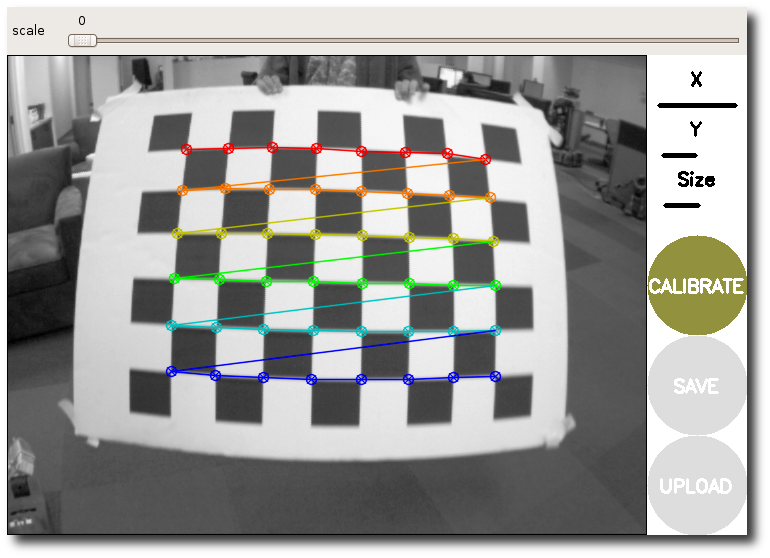
\includegraphics[width=0.8\textwidth]{./Bilder/Camera_Calibration_fig.png}\label{Calibration_of_Camera}
  \caption{Calibration of Camera\ref{Calibration_of_Camera}}
\end{figure}

For this master's thesis, the camera was calibrated and the parameters of the camera matrix can be found in the Table \ref{tab:meinetabelle}


\item \textbf{Extrinsic Parameters :} Extrinsic parameters are dependent on the camera position. The parameters are H and $\theta$. H is the distance between the camera and ground. $\theta$ is the camera tilt angle. These values must be measured because they have to be used for Inverse Perspective Mapping. The extrinsic parameters of the camera can be found in the Table \ref{tab:meinetabelle}. 
 
\end{itemize}
  
\begin{figure}[H]
\centering
  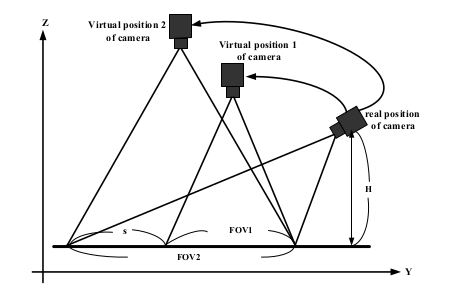
\includegraphics[width=0.8\textwidth]{./Bilder/Related_positions_of_the_camera.png}\label{Procedures_of_IPM_fig}
  \caption{Related Positions of the Camera \cite{IPM}}
\end{figure}

 As seen at Figure \ref{Procedures_of_IPM_fig}, the camera on the car has field of view 2(FOV2) at the real position of the camera but in this case, the view is not a bird's-eye view, so if the same FOV is to be observed from a bird's-eye view, IPM will virtually change the position to Virtual Position 2 of the camera. In this case, although the camera is at its real position, it will appear as though it is at Virtual Position 2. For that, the image coordinates must also be changed. Below, the steps of IPM calculations from the paper of \cite{IPM} will be detailed.
 
In the formula, the original image coordinates will be defined as (x,y), the destination image coordinates will be defined as ($x^*$,$y^*$), the distance between the ground and the camera will be defined as H, the focal length of camera will be defined as f, and the tilt angle of camera will be defined as $\theta$.
 
\begin{center}
 $x^* = H \frac{x sin \theta + f cos \theta}{-y cos \theta + f sin \theta}$ ;
 $y^* = H \frac{y sin \theta + f cos \theta}{-y cos \theta + f sin \theta}$ 
\end{center}

In this equation, the transformed component values of $x^*$ and $y^*$ may be less than or equal to zero. Because of 
this reason, a constant d is defined as $
\begin{vmatrix}
H(sin \theta + cos \theta)/(f sin \theta - cos \theta) 
\end{vmatrix}
$  + 1. This means that the coordinate point in the original source image has been mapped into the point of the destination image coordinate system. Below there is the proposed equation :
 
 \begin{center}
 $x^* = H \frac{x sin \theta + f cos \theta}{-y cos \theta + f sin \theta}$ + d ,
 $y^* = H \frac{y sin \theta + f cos \theta}{-y cos \theta + f sin \theta}$ + d ,
 where d = 
 $\begin{vmatrix}
 \frac{H(sin \theta + f cos \theta)}{f sin \theta - cos \theta}
 \end{vmatrix}$ + 1
\end{center}

\begin{figure}[H]
 \centering
  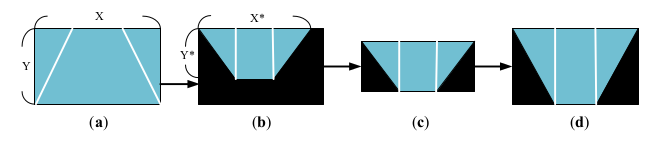
\includegraphics[width=1\textwidth]{./Bilder/Procedures_of_IPM.png}\label{Procedures_of_IPM}
  \caption{Procedures of IPM}
\end{figure}


%
\section{Edge Detection}\label{sec:Edge Detection}
%

Edge detectors are essential parts of most computer vision systems. Edge detectors dramatically decrease the amount of data to be processed and extract the useful parts of images. They work by detecting discontinuities in brightness. In this project, the edge detector was used in order to detect the lanes and to exclude unnecessary information from images. There are different methods for edge detection, but they can be grouped into two categories. They are :

\begin{itemize}

\item \textbf{Gradient method : } This method searches for the maximum and minimum in the first derivative of the image and with that, the edges can be found. For this method, the first order derivative filter must be used. For example : Sobel-Operator.
 
\item \textbf{Laplacian method : } This method searches for the zero crossing in the second derivative of the image and with that, the edges can be found. For this method, the second order derivative filter must be used. For example : Laplacian Filter. 
  
\end{itemize}
 
According to \cite{Machine_Vision},here are three steps of the edge detection algorithm. They are :

\begin{itemize}

\item \textbf{Filtering : } For edge detection, it is required to use a suitable smoothing filter. The filters sharpen the edges and ignore the unnecessary information. It is often utilized to improve the functioning of an edge detector against noise. The more filtering is applied, however, the greater the loss of edge strength.
 
\item \textbf{Enhancement : } To be able to better detect edges, changes in the intensity in the area surrounding a point must be determined. Pixels in which a significant change in intensity occurs are emphasized by enhancement, which is usually applied by calculating the gradient magnitude.
  
\item \textbf{Detection : } Though many points in an image have a nonzero value for the gradient, not all of these points are actually edges. Because only points with strong edge content are desired, a method must be applied to determine which points are actual edge points. Thresholding is often utilized to do so.
 
\end{itemize}

Well known smoothing filters are :

\begin{itemize}

 \item Sobel-Operator
 \item Canny Edge Detector
 \item Laplacian-Filter
 \item Prewitt-Operator
 
 \end{itemize}
 
In this master's thesis, the Sobel Operator was utilized, so it will be described in more detail.

%
\subsection{Sobel Operator}\label{sec:Sobel Operator}

The Sobel Operator, sometimes called the Sobel filter is one of the most used edge detectors in image processing and computer vision. The Sobel Operator uses vertical and horizontal masks. These masks used are odd-numbered square matrices and they are generally 3x3 matrices. Approximations of the derivatives for the horizontal changes and for the vertical changes are calculated by the operator by using two 3x3 kernels and convolving them with the original image. If A is defined as the source, if $G_{x}$ is an image which contains the horizontal derivative approximations at each point, and if $G_{y}$ is an imagine which contains the vertical derivative approximations at each point, then the calculations are:

\begin{center}

$  G_{x} = 
  \begin{bmatrix}
	+1 & 0 & -1 \\
	+2 & 0 & -2 \\
	+1 & 0 & -1 \\
   \end{bmatrix} * A  \quad
  G_{y} = 
  \begin{bmatrix}
	+1 & +2 & +1 \\
	0 & 0 & 0 \\
	+1 & -2 & -1 \\
  \end{bmatrix} * A		$

\end{center}

where * here denotes the 2-dimensional signal processing convolution operation.

Since the Sobel kernels can be decomposed as the products of an averaging and a differentiation kernel, they compute the gradient with smoothing. For example, \textbf{$G_{x}$}  can be written as

\begin{center}
$  \begin{bmatrix}
	+1 & 0 & -1 \\
	+2 & 0 & -2 \\
	+1 & 0 & -1 \\
   \end{bmatrix} =  \begin{bmatrix}
	1 \\
	2 \\
	1 \\
  \end{bmatrix} \begin{bmatrix}
	+1 & 0 & -1
  \end{bmatrix}
$
\end{center}


The x-coordinate is defined here as increasing in the 'right'-direction, and the y-coordinate is defined as increasing in the 'down'-direction. At each point in the image, the resulting gradient approximations can be combined to give the gradient magnitude, using:

\begin{center}
G = $\sqrt{ G_{x}^{2} + G_{y}^{2} }$
\end{center}

Using this information, we can also calculate the gradient's direction:

\begin{center}
$\theta = atan(\dfrac{G_{y}}{G_{x}})$
\end{center}

where, for example, $\theta$ is 0 for a vertical edge which is lighter on the right side.\cite{Sobel_Operator}


\begin{figure}[H]
  \centering
  \subfloat[Original Image]{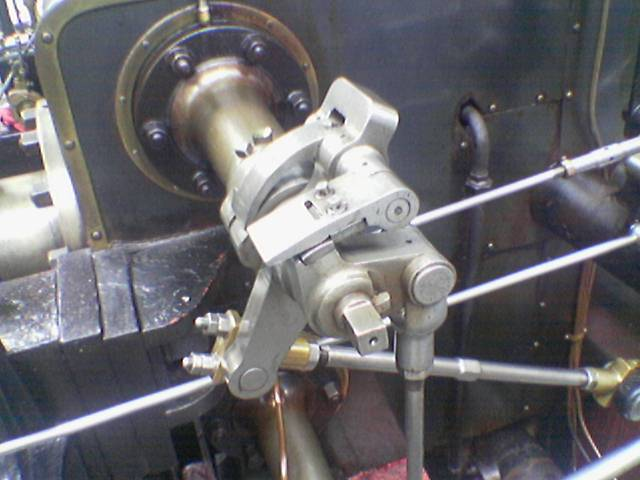
\includegraphics[width=0.4\textwidth]{./Bilder/Sobel_Original.png}\label{fig:f1}}
  \hfill
  \subfloat[Sobel Operator applied Image]{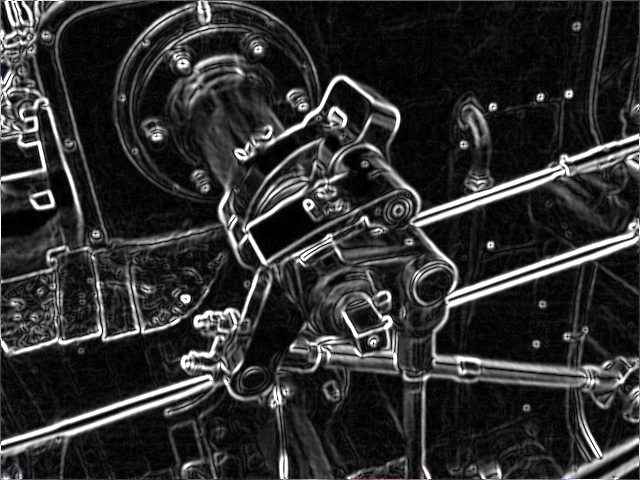
\includegraphics[width=0.4\textwidth]{./Bilder/Sobel_Operator.png}\label{fig:f2}}
  \caption{Sobel Operator\cite{Sobel_Operator}}
\end{figure} 


In this master's thesis, the Sobel Operator function in OpenCV was used. Before the Sobel operator was used, in order to reduce the noise, the 'GaussianBlur' function was used. As can perhaps be inferred from the name, the 'GaussianBlur' function blurs the image using a Gaussian filter. In order to apply the 'GaussianBlur' function, the following command must be run.

 \begin{center}
  
void GaussianBlur(InputArray src, OutputArray dst, Size ksize, double sigmaX, double sigmaY=0, int borderType=BORDER$\_$DEFAULT )

  \end{center}

The parameters of the function will be described in detail.\cite{GaussianBlur}
 
\begin{itemize}

\item \textbf{src : }Input image, which can have any number of channels but the depth of which must be one of the following: CV$\_$8U, CV$\_$16U, CV$\_$16S, CV$\_$32F and CV$\_$64F.
 
\item \textbf{dst : }Output image, which must be the same size and type as the input image.

\item \textbf{ksize : }Gaussian kernel size. This size shows the width and height of the Gaussian kernel. These sizes must not be the same value and the values must be odd and positive.

\item \textbf{sigmaX : }Gaussian kernel standard deviation in the X direction.

\item \textbf{sigmaY : }Gaussian kernel standard deviation in the Y direction.

\item \textbf{borderType : }Pixel extrapolation method.

\end{itemize}

After the Gaussian Filter is applied, the picture must be converted from color to grayscale. For that, there is a small function in OpenCV. With the following command, a color picture can be converted easily to grayscale.

 \begin{center}
 
void cvtColor(InputArray src, OutputArray dst, int code, int dstCn=0 )

 \end{center}
 
 The parameters of the function will be described in detail.
 
 \begin{itemize}

\item \textbf{src : }Input image
 
\item \textbf{dst : }Output image which is the same size and depth with input image.

\item \textbf{code : }Color space conversion code(here used CV$ \_ $BGR2GRAY).

\item \textbf{dstCn : }Number of channels in the destination image.


\end{itemize}

Before the Sobel operator is used, the Gaussian Filter must be applied and the image must be converted to gray scale. After this, the image is ready for Sobel operator to be applied. In order to calculate the 'derivatives' in the x and y directions, the following command must be run twice because gradient X and gradient Y must be calculated separately.

 \begin{center}

void Sobel(InputArray src, OutputArray dst, int ddepth, int dx, int dy, int ksize=3, double scale=1, double delta=0, int borderType=BORDER$\_$DEFAULT )

 \end{center}
 
 The parameters of the function will be described in detail.
 
  \begin{itemize}

\item \textbf{src : }Input image.

\item \textbf{dst : }Output image which is in the same size and depth with input image.

\item \textbf{ddepth : }The depth of the output image.

\item \textbf{xorder : }Order of the derivative x.

\item \textbf{yorder : }Order of the derivative y.

\item \textbf{ksize : }Size of the extended Sobel kernel; it must be 1, 3, 5, or 7.

\item \textbf{scale,delta and borderType : }Optional values. In this project, the default values were used.

  \end{itemize}

The last step of the application of the Sobel operator is approximating the gradient by adding both directional gradients. In the previous step, the gradients of the x and y coordinates were calculated separately. With following command, the weighted sum of these two gradients must be calculated.\cite{addWeighted}

 \begin{center}
 
void addWeighted(InputArray src1, double alpha, InputArray src2, double beta, double gamma, OutputArray dst, int dtype=-1)
 
  \end{center}
  
  The parameters of the function will be described in detail.
  
    \begin{itemize}

\item \textbf{src1 : }First input array.

\item \textbf{alpha : }Weight of the first array elements.

\item \textbf{src2 : }Second input array. This array must have the same size and channel number of the first input array.

\item \textbf{beta : }Weight of the second array elements.

\item \textbf{dst : }Output array, which has the same size and channel number of the the input arrays.

\item \textbf{gamma : }Scalar added to each sum.

\item \textbf{dtype : }Optional depth of the output array.

 \end{itemize}
 
%
\subsection{Canny Edge Detector}\label{sec:Canny Edge Detector}

Canny edge detector was developed in 1986 and called with the name of its developer John F. Canny. Canny edge detector is also so popular edge detector like Sobel operator. Canny edge detector is a multi-stage algorithm and it can be analyzed in 5 different stages.\cite{Canny_Edge_Detector2}

\begin{enumerate}
\item \textbf{Noise Reduction : } To get so stabile lane detection results, we have to reduce/remove all noise from frames. Lane detection without filtering out the noise can cause false detection. Gaussian filter is used for removing noise in the frames. Gaussian filter blurs images and removes detail and noise. The size of Gaussian filter kernel must be (2k+1)x(2k+1). It is important to choose the size of Gaussien filter because if the size of kernel is larger, detector's sensitivity to noise is lower but on the other hand, with the increase in size of the Gaussian filter kernel, the localization error in the edge detection will also increase slightly. \cite{Canny_Edge_Detector}



\item \textbf{Finding Intensity Gradient of the Image : } Essentially, the Canny algorithm locates edges in image where the grayscale intensity changes most starkly. In order to find these areas, the gradients of the image must be determined. In order to determine the gradients at each pixel in the smoothed image, the Sobel operator is applied. The Sobel operator has already been thoroughly discussed in section \ref{sec:Sobel Operator}.

\item \textbf{Non-maximum Suppression : } Non-maximum suppression is an edge thinning technique which is used as an intermediate step in many computer vision algorithms. The image is scanned along the image gradient direction, and pixels that are not part of the local maxima are set to zero. This way, all image information that is not part of the local maxima is effectively suppressed.

\item \textbf{Double Thresholding : } The edge pixels remaining after applying non-maximum suppression provide a more accurate depiction of real edges in an image. Despite this, there are still some remaining edge pixels resulting from noise and color variation. Therefore, it is necessary to filter out edge pixels with a weak gradient value while preserving edge pixels with a high gradient value. In order to do this, high and low threshold values must be selected. Edge pixels are marked as strong edge pixels when gradient values are higher than the high threshold value. They are marked as weak edge pixels when gradient values are lower than the high threshold value and higher than the low threshold value. They are suppressed when their values are lower than the low threshold value. The two threshold values are determined empirically and are dependent on the content of a given image.


\item \textbf{Hysteresis Thresholding : } Hysteresis Thresholding is the last part of Canny Edge Detector. Until this step, strong edge pixels are extracted from the true edges but there are also some weak edge pixels, some of them are extracted from true edges and some of them are extracted from some noise. So the weak edge pixels which are extracted from true edge, should be strong edge pixels and the weak edge pixels which are extracted from noises must be removed. If there is a weak edge pixel, 8 neighbour pixels of that weak edge pixel is checked and if at least, one pixel of these neighbour pixels is a strong edge pixel then, this weak edge pixels stay as edges in the end picture. 

\end{enumerate}


\begin{figure}[H]
  \centering
  \subfloat[Original Image]{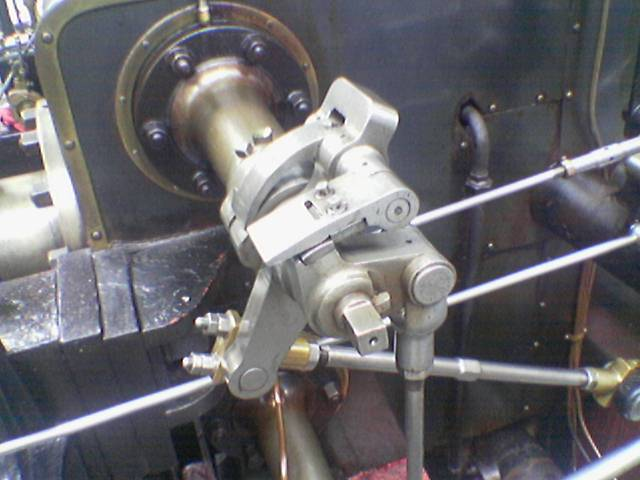
\includegraphics[width=0.4\textwidth]{./Bilder/Sobel_Original.png}\label{fig:f1}}
  \hfill
  \subfloat[Canny Edge Detector applied Image]{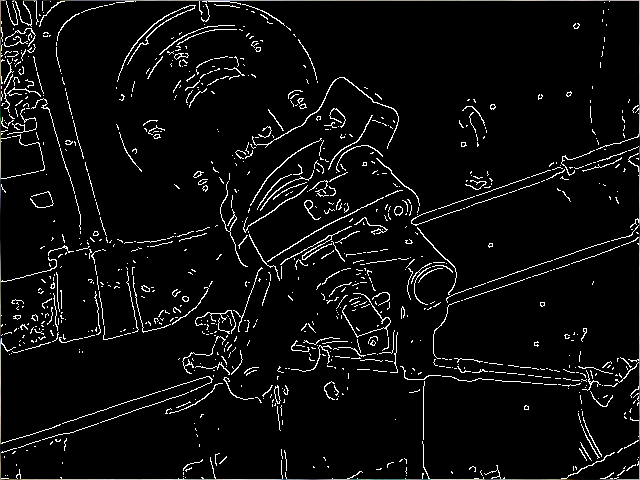
\includegraphics[width=0.4\textwidth]{./Bilder/Canny_Edge_Detector.png}\label{fig:f2}}
  \caption{Canny Edge Detector\cite{Canny_Edge_Detector}}
\end{figure} 

The Canny Edge Detector is also a function in OpenCV. As is the case with the Sobel Operator, before the Canny Edge Detector is used, a filter should be applied (for example, the Gaussian Filter) and the image must be converted to gray scale. With the following command, the Canny Edge Detector can be run in OpenCV.\cite{Canny_Edge_Detector3}

 \begin{center}
 
void Canny(InputArray image, OutputArray edges, double threshold1, double threshold2, int apertureSize=3, bool L2gradient=false)

 \end{center}
 
 The parameters of the function will be described in detail.\cite{Canny_Edge_Detector3}
 
     \begin{itemize}

\item \textbf{image : }Input image, which has to have an 8-bit single channel.

\item \textbf{edges : }Output image, which is the same size and type.

\item \textbf{threshold1 : }First threshold of the hysteresis procedure.

\item \textbf{threshold2 : }Second threshold of the hysteresis procedure.

\item \textbf{apertureSize : }Size of the extended Sobel kernel.

\item \textbf{L2gradient : }A flag for image gradient magnitude.

\end{itemize}
 
%
\section{Hough-Transformation}\label{sec:Hough-Transformation}
%
In order to isolate features of a particular shape in an image, a method called the Hough Transformation can be utilized. The Hough Transformation which is universally used today was further developed by Richard O. Duda and Peter E. Hart in 1972, although a more rudimentary version had been patented by Paul Hough in 1962.\cite{Hough_Transformation} In computer vision, it is often necessary to detect simple edges like straight lines, curves, and ellipses. As a result, this technique is used often in computer vision and image processing. The Hough Transformation is used mostly after an edge detection algorithm. There are actually variations of the Hough Transformation. In this master's thesis, two variations of the Hough Transformation were used. They are:

\begin{itemize}

\item \textbf{Standard Hough Line Transformation : }This type of Hough Transformation is used mostly for detecting straight lines. How the Standard Hough Transformation works will be explained in detail and as a result, why it is more suitable for detecting straight lines will become more clear.

\item \textbf{Probabilistic Hough Transformation : }This type of Hough Transformation is suitable for both straight lines and curves, so in this master's thesis, the Probabilistic Hough Transformation was used for detecting lanes. How the Probabilistic Hough Transformation works will also be explained.

\end{itemize}
%
\subsection{Standard Hough Line Transformation}\label{sec:Standard Hough Line Transformation}
%
The Standard Hough Line Transformation, which is also called the Linear Hough Transformation, is used mostly for detecting straight lines. There are many different formulas to represent a line segment analytically. A convenient formula for representing a line in an Image(Cartesian) space is :

  \begin{center}

$ \rho = x cos \theta + y sin \theta $

  \end{center}
  
In this equation, \textit{$ \rho $} is the length of a normal from the origin to the line and \textit{$ \theta $} is the orientation of \textit{r} with respect to the x-axis.
 
 
 \begin{figure}[H]
 \centering
  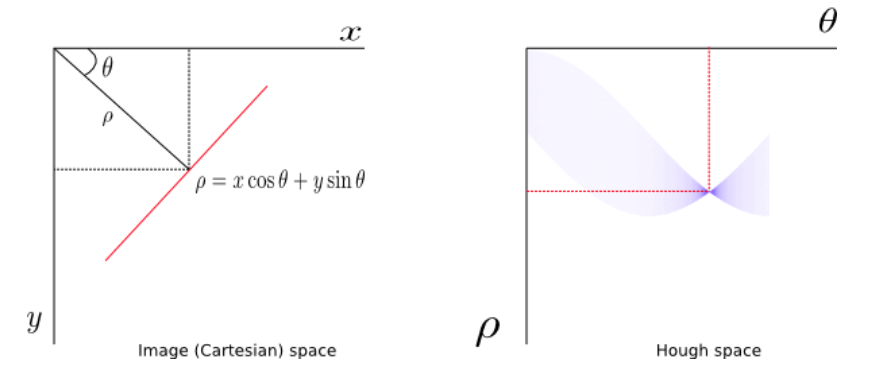
\includegraphics[width=0.8\textwidth]{./Bilder/Standard_Hough_Line_Transformation.png}\label{Standard_Hough_Line_Transformation_fig}
  \caption{Standard Hough Line Transformation\cite{Standard_Hough_Transformation}}
\end{figure}
 
 In the left side of Figure \ref{Standard_Hough_Line_Transformation_fig}, a line is shown in an Image (Cartesian) space and on the right side of same Figure, the same line is shown in its transformed state in the Hough space. A point in the Image (Cartesian) space is transformed into a sinusoidal curve in the Hough space. A line can be defined as a set of points, so a line is transformed into a set of sinusoids intersecting at a point in the Hough space. In this case, detecting points in the Hough space also means detecting the lines in the Cartesian space. After detecting points in the Hough Space, the points must be inversely transformed in order to get the corresponding lines in the Cartesian space.
 
\emph{\color{red}Although Hough transform (HT) has been widely used in curve detection, it has two major drawbacks: First, for each nonzero pixel in the image, the parameters for the existing curve and redundant ones are both accumulated during the voting procedure. Second, the accumulator array (or Hough space) is predefined in a heuristic way. The more accuracy needed, the higher parameter resolution should be defined. These two needs usually result in a large storage requirement and low speed for real applications. Therefore, RHT was brought up to tackle this problem.}

In this master's thesis, in order to detect the Hough lines, the function of \textit{cv2.HoughLines()} in OpenCV was used. The function is:

  \begin{center}
  
$HoughLines(dst, lines, \rho, \theta, threshold, srn, stn )  $

  \end{center}

The parameters of the function will be described in detail.\cite{Standard_Hough_Transformation2}
 
\begin{itemize}

\item \textbf{dst : }Output of the edge detector. It should be a grayscale image (although in fact it is a binary one).
 
\item \textbf{lines : }A vector that will store the parameters ($ \rho $, $ \theta $) of the detected lines. At the end of the Standard Hough Line Transformation, only the $ \rho $ and $ \theta $ values will be returned, so only straight lines can be drawn in OpenCV.

\item \textbf{$ \rho $ : }The resolution of the parameter $ \rho $ in pixels. In this master's thesis, \textbf{1 pixel} was used.

\item \textbf{$ \theta $ : }The resolution of the parameter $ \theta $ in radians. In this master's thesis, \textbf{180 degree}(CV$ \_ $PI) was used.

\item \textbf{threshold : }The minimum number of intersections to 'detect' a line.

\item \textbf{srn and stn : }Both of these parameters are for the multi-scale Hough transformation. srn is a divisor for the distance resolution $ \rho $ and stn is a divisor for the distance resolution $ \theta $. Default values of both parameters are zero.

\end{itemize}

%
\subsection{Probabilistic Hough-Transformation}\label{sec:Probabilistic Hough-Transformation}
%

\emph{\color{blue}Probabilistic Hough Transformation is also called Randomized Hough Transformation, is a variant of the Standard Hough Transformation.}Hough Transformation is computationally expensive. Probabilistic Hough Transformation is an optimization of Standard Hough Transformation which does not analyze all points in the image. Instead, it looks at only a random subset of points sufficient for line detection. \emph{\color{blue}In order to apply Probabilistic Hough Transformation, the threshold must be decreased.} \emph{\color{red}Probabilistic Hough Transformation is commonly used to detect curves (straight line, circle, elipse,etc.) }



\emph{\color{red}The basic idea of Hough transform (HT) is to implement a voting procedure for all potential curves in the image, and at the termination of the algorithm, curves that do exist in the image will have relatively high voting scores. Randomized Hough transform (RHT) is different from HT in that it tries to avoid conducting the computationally expensive voting process for every nonzero pixel in the image by taking advantage of the geometric properties of analytical curves, and thus improve the time efficiency and reduce the storage requirement of the original algorithm.}

  \begin{center}
  
$HoughLinesP(dst, lines, \rho, \theta, threshold, minLinLength, maxLineGap )  $

  \end{center}

The parameters of the function will be described in detail.\ref{Standard_Hough_Transformation2}
 
\begin{itemize}

\item \textbf{dst : }Output of the edge detector. It should be a grayscale image (although in fact it is a binary one).
 
\item \textbf{lines : }A vector that will store the parameters ($ x_{start} $, $ y_{start} $, $ x_{end} $, $ y_{end} $) of the detected lines.

At the end of the Probabilistic Hough Transformation, the end points of detected lines will be returned. With the Probabilistic Hough Transformation in OpenCV, straight lines can be detected. In addition, the small straight lines in other shapes can be combined, and with this technique, all shapes can be detected.  

In this master's thesis, all lanes were detected with Probabilistic Hough Transformation. However, instead of Hough Lines, the points which were returned as the result of Probabilistic Hough Transformation were used.

\item \textbf{$ \rho $ : }The resolution of the parameter $ \rho $ in pixels. In this master's thesis, \textbf{1 pixel} was used.

\item \textbf{$ \theta $ : }The resolution of the parameter $ \theta $ in radians. In this master's thesis, \textbf{1 degree}(CV$ \_ $PI/180) was used.

\item \textbf{threshold : }The minimum number of intersections to 'detect' a line.

\item \textbf{minLinLength : }The minimum number of points that can form a line. Lines with less than this number of points are disregarded.

\item \textbf{maxLineGap : }The maximum gap between two points to be considered in the same line.

\end{itemize}



%
\section{K-Nearest Neighbors Algorithm}\label{sec:K-Nearest Neighbors Algorithm}
%
K-Nearest Neighbor(KNN) is an non-parametric lazy learning algorithm. The non-parametric technique means that it doesn't make any assumptions on the underlaying data distribution. In the definition of KNN, the term 'lazy learning algorithm' is used. It means it doesn't use the data training points to do any generalization. In other words, there is no explicit training phase or it is very minimal.  It also means that the training phase is pretty fast. Most of the lazy algorithms - especially KNN - make decisions based on the entire training data set. On the other hand, KNN is one of the top 10 data mining algorithms\cite{k_nearest_neighbors}.

\begin{figure}[H]
 \centering
  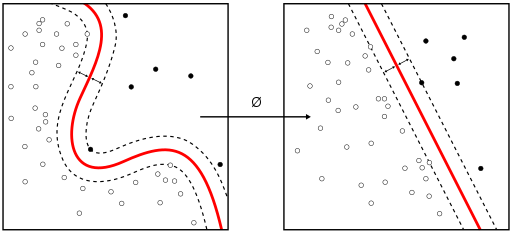
\includegraphics[width=0.8\textwidth]{./Bilder/k-nearest-neighbors.png}\label{Procedures_of_IPM}
  \caption{K-Nearest-Neighbors Algorithm\cite{k_nearest_neighbors_wikipedia}}
\end{figure}

\emph{\color{red}By using the training dataset directly, KNN makes predictions. By searching the entire training set for the K most similar instances (the neighbors) and summarizing the output variable for those K instances, predictions are made for a new instance (x). {For regression this might be the mean output variable, in classification this might be the mode (or most common) class value.} Distance measure methods are used for the determining which of the K instances in the training dataset are the nearest to a new input. There are so many different distance measure methods. Some of them are :}

\begin{itemize}

\item \textbf{Euclidean Distance : }It is one of the most popular methods for distance measure. In this method, the square root of the sum of the squared differences between a new point and an existing point is calculated.

  \begin{center}
  
\textbf{Euclidean} $ \sqrt{\sum_{i=1}^k  (x_{i} - y_{i})^2 } $

  \end{center}
  


\item \textbf{Manhattan Distance : }It is called also City Block Distance. It calculates the distance between real vectors using the sum of their absolute difference.

  \begin{center}
  
\textbf{Manhattan} $\sum_{i=1}^k \begin{vmatrix}x_{i} - y_{i} \end{vmatrix}$

  \end{center}
  

\item \textbf{Minkowski Distance : }The Minkowski distance is a metric in a normed vector space which can be considered as a generalization of both the Euclidean distance and the Manhattan distance.
  
  \begin{center}
  
\textbf{Minkowski} $ (\sum_{i=1}^k (\begin{vmatrix}x_{i} - y_{i} \end{vmatrix})^q)^{1/q}$

  \end{center}

\end{itemize}

There are also some other distance measure methods like Tanimoto, Jaccard, Mahalanobis, cosine distance and so on. It must be decided which distance measure method should be used according the properties of the dataset. For example, if the input variables are similar in type (e.g. all measured widths and heights), the Euclidean distance measure method is good. However, if the input variables are not similar in type (such as age, gender, height, etc.), the Manhattan distance measure method is better than the Euclidean measure distance method.



The K-Nearest Neighbors Algorithm has advantages and disadvantages. According to \cite{k_nearest_neighbors_adv_disadv},the main advantages of KNN are simplicity, effectiveness, intuitiveness and competitive classification performance in many domains. On the other hand, KNN can have poor run-time performance when the training set is large. It is very sensitive to irrelevant or redundant features because all features contribute to the similarity and thus to the classification. The computation cost is also quite high because we need to compute distance of each query instance to all training samples. 

K-Nearest Neighbors Algorithm is also a function in OpenCV. The following command shows the usage of the KNN function in OpenCV.

\begin{center}

void flann::Index$\_$<T>::knnSearch(const vector<T>$\&$ query, vector<int>$\&$ indices, vector<float>$\&$ dists, int knn, const SearchParams$\&$ params)

\end{center}

The parameters of the function will be described in detail.\cite{k_nearest_neighbors_OpenCV}

\begin{itemize}

\item \textbf{query : }The query point.

\item \textbf{indices : }The indices of the KNN are found in this vector.

\item \textbf{dists : }The distances of the KNN are found in this vector.

\item \textbf{knn : }Number of nearest neighbors to search for.

\item \textbf{params : }There are some different optional parameters, which can be used in this function.

\end{itemize}


%
\section{Curve Fitting}\label{sec:Curve Fitting}

\emph{\color{red}Curve fitting is used to find the 'best fit' line or curve for a series of data points. Curve fitting produces mostly mathematical equations that can be used to find points anywhere along
the curve.\cite{Curve_Fitting}} They are several different types of curve fitting. Some of them are: linear, exponential, polynomial, exponential, power, logarithmic, etc. In this master thesis, polynomial curve fitting was used. Polynomial curve fitting differs from order of the polynomial. Polynomial curve fittings are called different names depending on their orders. First order polynomial curve fittings are called linear regression, second order as quadratic regression, and third order as cubic regression.


\begin{figure}[H]
 \centering
  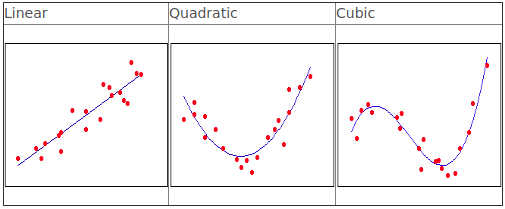
\includegraphics[width=0.8\textwidth]{./Bilder/Curve_Fitting_Polynomial.png}\label{Curve_Fitting_Polynomial}
  \caption{Types of Polynomial Curve Fitting\cite{Curve_Fitting_Polynomial}}
\end{figure}


In this master's thesis, curve fitting is used for getting the best mathematical descriptions of lanes. Curve fitting uses the Hough points which appear on the lanes as input, and give a mathematical equation as output. First order polynomial curve fitting is more suitable for defining straight lines and second order polynomial curve fitting is more suitable for defining curves. There are both straight and curved lanes, so first order polynomial curve fitting is not sufficient for our project. Accordingly, in this master's thesis, second order polynimal curve fitting is used.

There are so many different methods for curve fitting. One of the most famous methods is the least squares method, which is also the method utilized in this master's thesis. Next, how a polynomial curve fitting is generated using the least squares method will be described.

\emph{\color{blue}A data set can be mostly expressed the relationship between variable with an equation which is mostly representated with a $k^{th}$ order polynomial. The general description of $ k^{th} $ is :}

\begin{center}
y = $ a_{k}x^{k} + ... + a_{1}x + a_{0} + \epsilon $ 
\end{center}

The general polynomial regression model with the error $\epsilon$ typically provides an estimate rather than an implicit value of the dataset for any given value of x. A data set which has N data points can be described with the maximum order of the polynomial which is k = N - 1, but the lowest possible order of the polynomial is generally chosen.

The aim of the least squares' method is to minimize the variance between dataset values and estimated values from the polynomial equation.

In order to determine the coefficients of the polynomial regression model ($ a_{k}, a_{k-1}, ..., a_{1} $) must be solved the following linear equations.

\begin{center}
 $
 \begin{bmatrix}
N & $$\sum_{i=1}^{N} x_{i}$$ & $\dots$ & $$\sum_{i=1}^{N} x_{i}^{k}$$ \\
$$\sum_{i=1}^{N} x_{i}$$ & $$\sum_{i=1}^{N} x_{i}^2$$ & $\dots$ & $$\sum_{i=1}^{N} x_{i}^{k+1}$$ \\
$\vdots$ & $\vdots$ & $\vdots$ & $\vdots$ \\
$$\sum_{i=1}^{N} x_{i}^{k}$$ & $$\sum_{i=1}^{N} x_{i}^{k+1}$$ & $\dots$ & $$\sum_{i=1}^{N} x_{i}^{2k}$$ \\

\end{bmatrix}  \begin{bmatrix}
	 a_{0}  \\
	 a_{1}  \\
	 \vdots  \\
	 a_{k}  \\
  \end{bmatrix} = 
  \begin{bmatrix}
	 $$\sum_{i=1}^{N} y_{i}$$  \\
	 $$\sum_{i=1}^{N} x_{i}y_{i}$$  \\
	 \vdots  \\
	 $$\sum_{i=1}^{N} x_{i}^{k}y_{i}$$  \\
  \end{bmatrix}
$ 
\end{center}

The equations in the stardard form of Ma = b can be solved with many different methods. In this master's thesis, \textit{Cramer's Rule} was used to solve for the polynomial coefficients of curve fitting. With the help of the determinants of the square matrix, M can be solved for in any linear system of equations in order to find the coefficients. Each of the coefficients $a_{k}$ may be determined using the following equation :

\begin{center}
$a_{k} = \dfrac{det(M_{i})}{det(M)}$
\end{center}

In order to find the coefficients of polynomial curve fitting, we have to use the equation shown above, so the determinate of $ M_{i} $ must be divided by the determinate of M. Above, the equation Ma = b was shown, so the determinate of the M matrix can be calculated. However, for the determinate of $ M_{i} $ matrix, the M matrix must be modified. To find the $ M_{i} $ matrix, the $ i^{th} $ column must be replaced with the column vector b, which was used in the equation Ma = b. For example, if the $ M_{0} $ matrix is to be determined, the M matrix must be modified like at the following\cite{Curve_Fitting2} :


\[
 M = \begin{bmatrix}
N & $$\sum_{i=1}^{N} x_{i}$$ & $\dots$ & $$\sum_{i=1}^{N} x_{i}^{k}$$ \\
$$\sum_{i=1}^{N} x_{i}$$ & $$\sum_{i=1}^{N} x_{i}^2$$ & $\dots$ & $$\sum_{i=1}^{N} x_{i}^{k+1}$$ \\
$\vdots$ & $\vdots$ & $\vdots$ & $\vdots$ \\
$$\sum_{i=1}^{N} x_{i}^{k}$$ & $$\sum_{i=1}^{N} x_{i}^{k+1}$$ & $\dots$ & $$\sum_{i=1}^{N} x_{i}^{2k}$$ \\

\end{bmatrix} \quad
 M_{0} = \begin{bmatrix}
$$\sum_{i=1}^{N} y_{i}$$ & $$\sum_{i=1}^{N} x_{i}$$ & $\dots$ & $$\sum_{i=1}^{N} x_{i}^{k}$$ \\
$$\sum_{i=1}^{N} x_{i}y_{i}$$ & $$\sum_{i=1}^{N} x_{i}^2$$ & $\dots$ & $$\sum_{i=1}^{N} x_{i}^{k+1}$$ \\
$\vdots$ & $\vdots$ & $\vdots$ & $\vdots$ \\
$$\sum_{i=1}^{N} x_{i}^{k}y_{i}$$ & $$\sum_{i=1}^{N} x_{i}^{k+1}$$ & $\dots$ & $$\sum_{i=1}^{N} x_{i}^{2k}$$ \\

\end{bmatrix}
\]

In this master's thesis, the $ 2^{nd} $ order polynomial equation is used, so only the values of $ a_{0}, a_{1} and a_{2} $ must be calculated. To understand curve fitting better, we are going to develop the $ 2^{nd} $ order polynomial curve fit for the given dataset.

\begin{center}
  \begin{tabular}{ | c | c | c | c | c | c | c |}
    \hline
    x & -3  &  -2  &  -1  & -0.2  &  1  &  3 \\ \hline
    y & 0.9 &  0.8 &  0.4 &  0.2  & 0.1 &  0 \\
    \hline
  \end{tabular}
\end{center}

\[
 M = \begin{bmatrix}
6 & -2.2 & 24.04 \\
-2.2 & 24.04 & -8.008 \\
24.04 & -8.008 & 180.0016 \\

\end{bmatrix} \quad
 M_{0} = \begin{bmatrix}
2.4 & -2.2 & 24.04 \\
-4.64 & 24.04 & -8.008 \\
11.808 & -8.008 & 180.0016 \\

\end{bmatrix} 
\]

\[
 M_{1} = \begin{bmatrix}
6 & 2.4 & 24.04 \\
-2.2 & -4.64 & -8.008 \\
24.04 & 11.808 & 180.0016 \\

\end{bmatrix} \quad
 M_{2} = \begin{bmatrix}
6 & -2.2 & 2.4 \\
-2.2 & 24.04 & -4.64 \\
24.04 & -8.008 & 11.808 \\

\end{bmatrix}
\]

$ a_{0} = \dfrac{det(M_{0})}{det(M)}   \Longrightarrow  a_{0} = \dfrac{ 2671.1962}{11661.2736} = 0.2291$  \vfill 
$ a_{1} = \dfrac{det(M_{1})}{det(M)} \Longrightarrow  a_{1} = \dfrac{ -1898.4602}{11661.2736} = -0.1628$  \vfill 
$ a_{2} = \dfrac{det(M_{2})}{det(M)} \Longrightarrow  a_{2} = \dfrac{ 323.7632}{11661.2736} = 0.0278$

In this case, the fitted curve function is : \vfill 
\begin{center}
y = 0.0278$x^{2} $ - 0.1628x +0.2291
\end{center}

\begin{figure}[H]
 \centering
  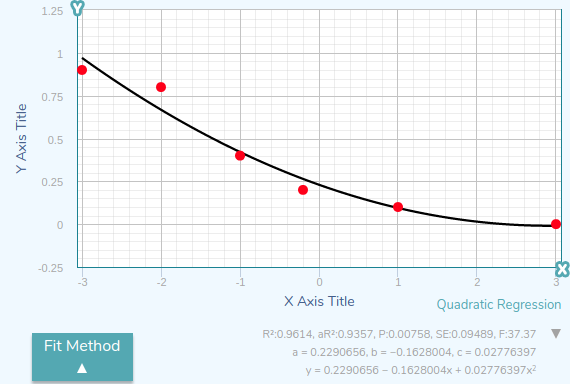
\includegraphics[width=0.8\textwidth]{./Bilder/Curve_Fitting.png}\label{Curve_Fitting}
  \caption{Curve Fitting\cite{Curve_Fitting_Plot}}
\end{figure}




%




